\documentclass[12pt]{article}

\input{physicsPream}

\usepackage{tabularx}
\usepackage{changepage}

\begin{document}

%----------BEGIN TITLEPAGE----------

\begin{titlepage}

  \title{Lab 4: Interferometry}
  \author{Ryan Wojtyla \\Partner: Akshath Wikramanayake}
  \date{November 6, 2018}

  \maketitle

  \begin{center}
    Abstract
  \end{center}

  \qq Throughout this lab, an interferometer is used to determine the indexes of
  refraction of several media. This was accomplished by measuring the phase
  difference between two versions of an incident beam split across two different
  paths; an uninterrupted path and a path through a subject medium. 

  \qq In the second experiment, the index of refraction of air at atmospheric
  pressure was calculated with a very small error to be \(n_{\text{atm}} =
  \num{1.0391} \pm \num{49.0e-9}\). In the third experiment, the index of
  refraction of glass was calculated with a rather high error to be \(n_g = 1.50 \pm
  10.3\).

  \thispagestyle{empty}

\end{titlepage}

%-----------END TITLEPAGE-----------

%----------BEGIN EXPERIMENT 1----------

\section{Experiment 1: Introduction to Interferometry}

\subsection{Objective}

\qq The purpose of the first experiment was to gain familiarity with the
interferometry equipment. The simple experiment of determining the wavelength of
the laser makes use of the basic setup without introducing too many extraneous
components. The relative simplicity of this experiment allows us to focus on
calibrating the interferometer and becoming well-versed in its operation.

\subsection{Theory}

\subsubsection{Part I: Wavelength}

\qq The first part of this experiment asks us to find the wavelength of the
incident laser. The interferometer has the effect of creating two beams incident
on the viewing screen, one having traveled a greater distance than the
other. Because the two beams have traveled different distances, they are out of
phase by a certain amount. The phase difference between the beams can be altered
by modifying the length of one of the beam's paths. This is accomplished by
rotating the micrometer to change the position of the adjustable mirror. As the
adjustable mirror is moved backward, the image of the waves' interference
pattern changes. When the phase difference completes half a revolution, the
image on the screen appears the same as before the micrometer was rotated. Each
time the image on the screen reverts back to its initial state, a fringe is said
to have passed by. Since only half a revolution results in a similar image, the
distance the mirror is adjusted is equal to half the wavelength of the
wave. This relationship is shown by

\begin{equation}
\label{eqn:wavelengthViaFringes}
  \lambda = 2 \frac{d_m}{N}
\end{equation}

where \(d_m\) is the distance traveled by the adjustable mirror and \(N\) is the
number of fringes that have passed. 

\subsubsection{Part II: Polarization}

\qq The second part of the experiment asks us to observe the effects of
polarizing the incident beam. A polarizer accepts incident light and only
transmits the components of that light whose orientation matches that of the
polarizer. With only one polarizer present, the image is slightly dimmer with any
angle. The image dims because a portion of the incident light is absorbed by the
polarizer, but because the incident light is not polarized, the same amount of
light is absorbed no matter the angle of the polarizer. With two polarizers,
however, the light can be completely blocked. Once the light is oriented in a
certain direction through the first polarizer, if the angle of the second
polarizer is perpendicular to that of the first, all of the light incident on
the second polarizer is absorbed, producing no transmission. Additionally, the
amount of light transmitted through the second polarizer is inversely
proportional to the angle of the second polarizer relative to that of the
first.  

\subsection{Equipment}

\begin{figure}[H]
  \label{pic:equip1}
  \begin{center}
    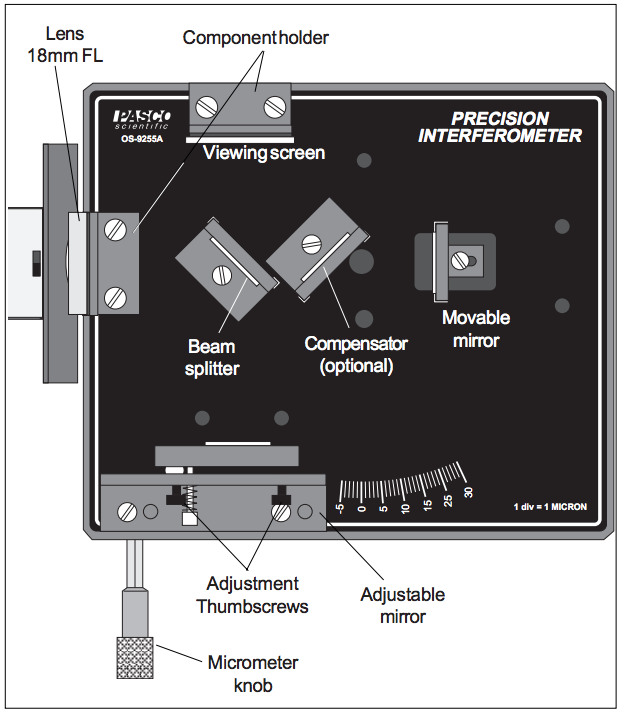
\includegraphics[scale=0.7]{equip1.png}
  \end{center}
  \caption{A diagram of the interferometer setup in Michelson mode; the
    configuration used for Experiment 1.}
\end{figure}

\begin{figure}[H]
  \label{tab:equip1List}
  \caption{The list of equipment used in Experiment 1.}
  \begin{center}
    \begin{tabular}{|c|c|c|c|}
      \hline
      Manufacturer & Model & Serial Number & Specifications \\
      \hline
      PASCO Scientific & Precision Interferometer & OS-9255A & n/a \\
      PASCO Scientific & Laser Alignment Bench    & OS-9172  & n/a \\
      PASCO Scientific & Component Holder         & OS-9256A & n/a \\
      PASCO Scientific & Polarizer (2)            & OS-9256A & n/a \\
      \hline
    \end{tabular}
  \end{center}
\end{figure}

\subsection{Procedures}

\subsubsection{Part I: Wavelength}

\qq The first part of the experiment involves measuring the wavelength of the
beam from the laser. Before beginning, the interferometer must be set up in Michelson
mode, and an interference pattern must be clearly visible on the viewing
screen. 

\qq To start off, the micrometer knob ought to be adjusted to a medium setting
of approximately \SI{50}{\micro\meter}. To minimize backlash during measuring,
turn the micrometer knob one full rotation counterclockwise, and to maximize
accuracy of measurement, continue turning counterclockwise until the zero on the
knob is aligned with the index mark. Record the micrometer reading, \(d_i\).

\qq Adjust the position of the viewing screen so that one of its marks
is aligned with the fringes of the interference pattern. This is the reference
mark. Slowly rotate the micrometer knob counterclockwise, and count the number
of fringes that pass the reference mark. Continue until at least 20 fringes are
counted. One fringe has passed by when the fringes return to the same position
before counting began. Record the final reading of the micrometer dial, \(d_f\).

\qq Calculate \(d_m = d_f - d_i\), the distance traveled by the adjustable
mirror, for the number of counted fringes, \(N\). Repeat these steps several
times.

\subsubsection{Part II: Polarization}

\qq With the same setup as above, place a polarizer between the laser and the
beam-splitter. Slowly rotate the polarizer to achieve several different
polarization angles, and observe any effects caused by this rotation. Move the
polarizer to in front of the movable mirror, and, again, observe the effects of
its rotation on the image on the screen.

\qq Now, place one polarizer in front of the fixed mirror and another in front
of the movable mirror. Rotate one polarizer, then the other, and observe any
effects this rotation has on the image on the screen.

\subsection{Data and Analysis}

\begin{figure}[H]
  \label{fig:exp1MicrometerMeasurements}
  \caption{The measurements of the micrometer while counting the fringes during
    Part I of Experiment 1.}
  \begin{adjustwidth}{-2cm}{}
    \begin{center}
      \begin{tabularx}{18cm}{|X|X|X|X|X|}
        \hline
        Initial Position (\(d_i\)) (\si{\micro\meter}) & 
        Final Position (\(d_f\)) (\si{\micro\meter}) &
        Mirror Movement \(d_m\) (\si{\micro\meter}) &
        Number of Fringes \(N\) & 
        Wavelength (\(\lambda\)) (\si{\nano\meter}) \\
        \hline
        52.5 \(\pm\) 0.05 & 53.2 \(\pm\) 0.05 & 0.7 \(\pm\) \num{0.0707} & 20 &
        70 \(\pm\) 7.07 \\
        \hline
      \end{tabularx}
    \end{center}
  \end{adjustwidth}
\end{figure}

\qq The distance the mirror traveled is found with \(d_m = d_f - d_i\), where
\(d_f\) is the final position of the micrometer and \(d_i\) is its initial
position. Both \(d_f\) and \(d_i\) have an error of \(\pm
\SI{0.05}{\micro\meter}\). Since \(d_i\) is subtracted from \(d_f\), the error
of \(d_m\), \(\delta d_m\), is found with

\begin{align*}
  \delta d_m &= \sqrt{\delta d_f^2 + \delta d_i^2} \\
  \delta d_m &= \sqrt{(0.05)^2 + (0.05)^2} \\
  \delta d_m &= \SI{0.0707}{\micro\meter} \\
\end{align*}

\qq The wavelength of the incident beam is found with

\begin{align*}
  \lambda &= \frac{2 d_m}{N} \\
  \lambda &= \frac{2 (0.7)}{(20)} \\
  \lambda &= \SI{70}{\nano\meter} \\
\end{align*}

Since \(N\) is the constant 20, and \(d_m\) is, net, multiplied by
\(\frac{1}{10}\), its error, \(\delta d_m\), must be similarly multiplied in
order to find the error in the wavelength, \(\delta \lambda\)

\begin{align*}
  \delta \lambda &= \frac{2 \delta d_m}{N} \\
  \delta \lambda &= \frac{2 (\num{0.0707})}{N} \\
  \delta \lambda &= \SI{0.00707}{\micro\meter} \\
\end{align*}

\subsection{Conclusion}

\qq While the error of the wavelength is low compared to the value of the
wavelength, it is not accurate. The actual wavelength is \SI{633}{\nano\meter},
but our measurement is for \SI{70}{\nano\meter}. Factors that limited the
accuracy of the micrometer measurements include placement of the final reading;
the dial can be difficult to read if the marker is in between markings on the
Vernier scale.

%-----------END EXPERIMENT 1-----------

%----------BEGIN EXPERIMENT 2----------

\section{Experiment 2: The Index of Refraction of Air}

\subsection{Objective}

\qq The purpose of this experiment is to use interferometry to determine the
index of refraction of air. This is accomplished by measuring the phase
difference of a split beam through two different media. In this case, the media
are normal air and a semi-evacuated chamber.   

\subsection{Theory}

\qq As discussed earlier, the wavelength of an incident light beam can be
determined by measuring the phase difference between two split versions of that
beam. The wavelengths of a light beam traveling through two different media are
related with Snell's Law, 

\begin{equation}
  \label{eqn:SnellsLawWavelength}
  \frac{\lambda_1}{\lambda_2} = \frac{n_2}{n_1} \\
\end{equation}

where \(\lambda_1\) and \(\lambda_2\) are the wavelengths of light traveling
through media with indexes of refraction \(n_1\) and \(n_2\), respectively. If
the first medium is a vacuum, then Equation \ref{eqn:SnellsLawWavelength} can be
rewritten as

\begin{equation}
  \label{eqn:SnellsLawVacuum}
  \lambda = \frac{\lambda_0}{n} \\
\end{equation}

where \(\lambda\) is the wavelength of the incident light beam after traveling
through a medium of index of refraction \(n\) with respect to its wavelength in
a vacuum, \(\lambda_0 = \SI{633}{\nano\meter}\). 

\qq At reasonably low pressures, the pressures at which this experiment takes
place, the index of refraction of a gas is linearly proportional to its
pressure. By slightly altering the pressure of a gaseous medium by a known,
proportional amount, the wavelength of a light beam traveling through the
altered medium will be affected by a similar relative amount.

\qq If the pressure of the medium is decreased, the wavelength of light passing
through it will be decreased by a proportional amount. This decrease in
wavelength manifests itself as a decrease in the number of fringes counted while
changing the pressure of the medium. Rewriting Equation
\ref{eqn:wavelengthViaFringes} for the number of fringes, the following two
equations can be obtained:

\begin{equation}
  \label{eqn:initialFringes}
  N_i = \frac{2d}{\lambda_i} \\
\end{equation}

\begin{equation}
  \label{eqn:finalFringes}
  N_f = \frac{2d}{\lambda_f} \\
\end{equation}

where \(d\) is now the length of the cell in which the pressure of the medium is
altered, \(N_i\) is the number of fringes counted when the light traveled through
the initial medium, and \(N_f\) is the number of fringes counted when the light
traveled through the modified, final medium. The difference between the number
of fringes, \(N\), can then be written as

\begin{equation}
  \label{eqn:totalFringes}
  N = \frac{2d}{\lambda_i} - \frac{2d}{\lambda_f} \\
\end{equation}

By applying Equation \ref{eqn:SnellsLawVacuum} to the initial and final
wavelengths in Equation \ref{eqn:totalFringes}, it can be rewritten as

\begin{equation}
  \label{eqn:totalFringesExpanded}
  N = \frac{2 d (n_i - n_f)}{\lambda_0} \\
\end{equation}

\qq Since the relationship between a medium's pressure and its index of
refraction is linear, the index of refraction of a medium is equal to the slope
of its \(n\) vs. \(P\) graph, where \(P\) is the pressure of the medium. The
equation for this graph can be found by rewriting Equation
\ref{eqn:totalFringesExpanded} as \(n_i - n_f = \frac{N \lambda_0}{2 d}\) and
multiplying both sides by the inverse of the pressure difference between the two
media, \(\frac{1}{P} = \frac{1}{P_i - P_f}\),

\begin{equation}
  \label{eqn:nVsP}
  \frac{n_i - n_f}{P_i - P_f} = \frac{N \lambda_0}{2 d} \frac{1}{P_i - P_f} \\
\end{equation}

\subsection{Equipment}

\begin{figure}[H]
  \label{fig:equip2}
  \begin{center}
    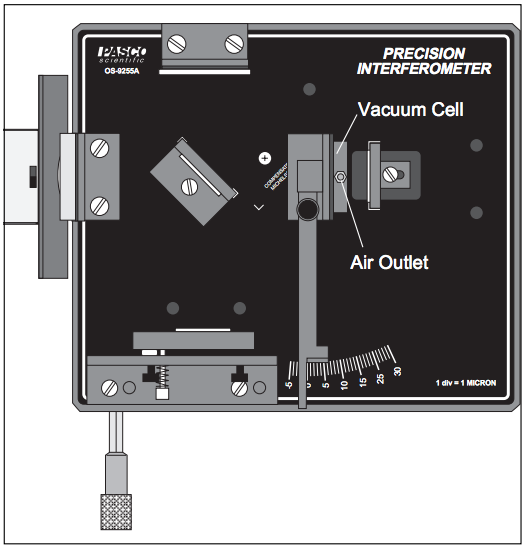
\includegraphics[scale=0.7]{equip2.png}
  \end{center}
  \caption{A diagram of the setup for Experiment 2. Since it is very similar to
    the setup of Experiment 1, only the components added to the interferometer
    for Experiment 2 have been labeled.}
\end{figure}

\begin{figure}[H]
  \label{tab:equip2List}
  \caption{A list of the equipment used in Experiment 2.}
  \begin{center}
    \begin{tabular}{|c|c|c|c|}
      \hline
      Manufacturer & Model & Serial Number & Specifications \\
      \hline
      PASCO Scientific & Precision Interferometer & OS-9255A & n/a \\
      PASCO Scientific & Laser Alignment Bench    & OS-9172  & n/a \\
      PASCO Scientific & Rotational Pointer       & OS-9256A & n/a \\
      PASCO Scientific & Vacuum Cell              & OS-9256A & thickness: \SI{8}{\milli\meter} \\
      PASCO Scientific & Vacuum Pump              & OS-9256A & n/a \\
      \hline
    \end{tabular}
  \end{center}
\end{figure}

\subsection{Procedures}

\qq Before starting, ensure that the interferometer is in Michelson mode,
properly aligned, and in the same configuration as Experiment 1. To set up the
interferometer for Experiment 2, place the rotational pointer between the
movable mirror and the beam-splitter, then attach the vacuum cell to the
magnetic backing of the rotational pointer. Attach the air hose to the vacuum
cell, then adjust the alignment of the fixed mirror so that the center of the
interference pattern is clearly visible on the viewing screen. 

\qq Ensure that the vacuum cell is at atmospheric pressure by flipping the
vacuum release toggle switch, and record this initial value of the vacuum cell's
pressure, \(P_i\). Slowly pump air out of the cell, and record the number of
fringes that pass the reference point on the viewing screen, \(N\). Continue pumping
until the vacuum pump's limit is reached, and record this final pressure,
\(P_f\). Repeat these steps to collect several trials' worth of data.

\subsection{Data and Analysis}

\qq The slope of the \(n\) vs. \(P\) graph, the \(m = \frac{N \lambda_0}{2 d}\) term
from Equation \ref{eqn:nVsP}, where \(N = 13\), \(\lambda_0 =
\SI{633}{\nano\meter}\), and \(d = \SI{8}{\milli\meter} \pm \SI{0.5}{\milli\meter}\) is

\begin{align*}
  m &= \frac{N \lambda_0}{2 d} \\
  m &= \frac{(13) (\num{633e-9})}{2 (\num{8e-3})} \\
  m &= \num{5.14e-4}
\end{align*}

\qq The general equation for determining the error in a function, \(y\), of
multiple variables, \(x_1, \ldots, x_n\), is

\begin{equation}
  \label{eqn:genErrProp}
  \delta y = y \sqrt{\left(\frac{\partial y}{\partial x_1} \delta x_1 \right)^2
    + \ldots + \left(\frac{\partial y}{\partial x_n} \delta x_n \right)^2} \\
\end{equation}

Applying Equation \ref{eqn:genErrProp} to \(m(d) = \frac{N \lambda_0}{2 d}\),
where \(d = \SI{8}{\milli\meter} \pm \SI{0.5}{\milli\meter}\), the error in the
slope, \(\delta m\), can be found:

\begin{align*}
  \delta m &= m \sqrt{\left( \frac{\partial m}{\partial d} \delta d \right) ^ 2}
  \\
  \delta m &= m \sqrt{ \left( \left( \frac{N \lambda_0}{2 d^2}
             \right) \delta d \right) ^ 2} \\
  \delta m &= (\num{5.14e-4}) \sqrt{ \left( \frac{(13)(\num{633e-9})}{2
             (\num{8e-3})^2} \delta d  \right) ^ 2} \\
  \delta m &= \num{1.65e-8} \\
\end{align*}

\qq The slope of the \(n\) vs. \(P\) graph is \(m = \num{5.14e-4} \pm
\num{1.65e-8}\). 

\begin{figure}[H]
  \label{gph:nVP}
  \begin{center}
    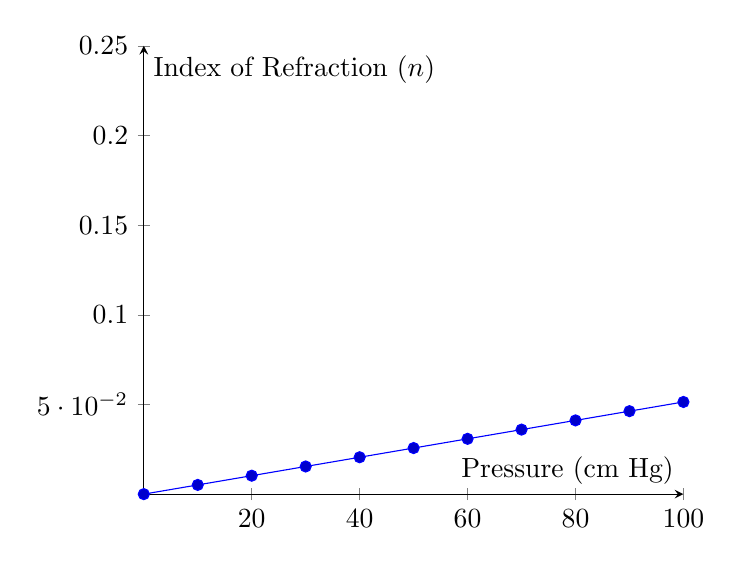
\begin{tikzpicture}
      \begin{axis}[
        xlabel={Pressure (cm Hg)},
        ylabel={Index of Refraction (\(n\))},
        axis lines = middle,
        xmin=0,
        xmax=100,
        ymin=0,
        ymax=0.25,
      ]
        \addplot+[
          domain=0:100, 
          samples=11
        ]
        {0.000514 * x};
      \end{axis}
    \end{tikzpicture}
  \end{center}
  \caption{The plot of \(n\) vs. \(P\).}
\end{figure}

\qq The index of refraction of air at a given pressure is found with

\begin{equation}
  \label{eqn:indexOfRefAir}
  n = 1 + n(P)
\end{equation}

where \(n(P) = m P = \num{5.14e-3} P\). Therefore, the index of refraction of
air at atmospheric pressure (\(P = 76 cmH Hg\)) is

\begin{align*}
  n_{\text{atm}} &= 1 + n(76) \\
  n_{\text{atm}} &= 1 + ((\num{5.14e-3})(76)) \\
  n_{\text{atm}} &= \num{1.0391} \\
\end{align*}

The error of the index of refraction of air is found by applying Equation
\ref{eqn:genErrProp} to Equation \ref{eqn:indexOfRefAir}:

\begin{align*}
  \delta n &= n \sqrt{\left( \frac{\partial n}{\partial m} \delta m \right) ^ 2}
  \\
  \delta n_{\text{atm}} &= (\num{0.0391}) \sqrt{\left( (P) (\num{16.5e-9})
                          \right) ^ 2} \\
  \delta n_{\text{atm}} &= (\num{0.0391}) \sqrt{\left( (76) (\num{16.5e-9})
                          \right) ^ 2} \\
  \delta n_{\text{atm}} &= \num{4.90e-8} \\
\end{align*}

\subsection{Conclusion}

\qq The property that the pressure of a gaseous medium is linearly related to
the medium's index of refraction was used to find the index of refraction of air
at atmospheric pressure. This was accomplished by plotting the index of
refraction of air as a function of the pressure of air. The slope of this linear
relationship was found to be \(m = \num{5.14e-4} \pm \num{1.65e-8}\). Therefore,
the index of refraction of air at atmospheric pressure, when \(P = 76 \text{cm
  Hg}\), is \(n_{\text{atm}} = 1.04\), a value very near 1.

\qq In order to test our assumption that the relationship between pressure and
index of refraction is linear, several trials would be conducted to verify our
results. The index of refraction of a gas also depends on temperature as it
depends on pressure. If temperature rather than pressure were used to find the
index of refraction of air, instead of evacuating an isolated chamber of air,
the temperature of the air in the chamber would be altered. 

%-----------END EXPERIMENT 2-----------

%----------BEGIN EXPERIMENT 3----------

\section{Experiment 3: The Index of Refraction of Glass}

\subsection{Objective}

\qq While the purpose of Experiment 2 is to measure the index of refraction of
air, a gas, the purpose of Experiment 3 is to measure the index of refraction of
glass, a solid. In order to achieve this, the wavelength of the light through
the material is, again, altered so that Snell's Law may be used to determine the
medium's index of refraction. In this case, the distance traveled by the light
through the medium in question is adjusted.

\subsection{Theory}

\qq Similar to Experiment 2, Snell's Law, Equation
\ref{eqn:SnellsLawWavelength}, is used to determine the index of refraction of
the medium through which the light passes. When light passes through a different
medium, its wavelength is altered. The longer the light has this altered
wavelength, as the distance traveled through the different medium increases, the
greater its phase shift from the unaltered beam. This change in phase shift is
quantified by counting the number of fringes passing the reference point, \(N\),
as the length of the medium is increased. The length of the medium is increased
by increasing the angle of the medium's plane with respect to the plane
perpendicular to the normal of the incident beam. 

\qq The total distance traveled by the light beam is represented as \(d =
d_a(\theta) + d_g(\theta)\), where \(d_a(\theta)\) and \(d_g(\theta)\) are the
distances traveled through air and glass, respectively, as functions of
\(\theta\), the angle between the plane of the glass and the plane perpendicular
to the normal of the beam. Keeping in mind that the index of refraction is also
different for each of the two media, the number of fringes that have passed the
reference point can be found by expanding Equation \ref{eqn:initialFringes} to
account for the change in medium:

\begin{equation}
  \label{eqn:fringesAirAndGlass}
  N = \frac{2 n_a d_a(\theta) + 2 n_g d_g(\theta)}{\lambda_0} \\
\end{equation}

where \(n_a\) and \(n_g\) are the indexes of refraction of air and glass
respectively and \(\lambda_0\) is the wavelength of the
incident beam in a vacuum. Equation \ref{eqn:fringesAirAndGlass} can then be
solved for the index of refraction of the glass, \(n_g\):

\begin{equation}
  \label{eqn:indexRefGlass}
  n_g = \frac{(2 t - N \lambda_0) (1 - \cos{(\theta)})}{2 t (1 - \cos{(\theta)})
  - N \lambda_0} \\
\end{equation}

where \(t\) is the thickness of the glass through which the light travels.

\subsection{Equipment}

\begin{figure}[H]
  \label{fig:equip3}
  \begin{center}
    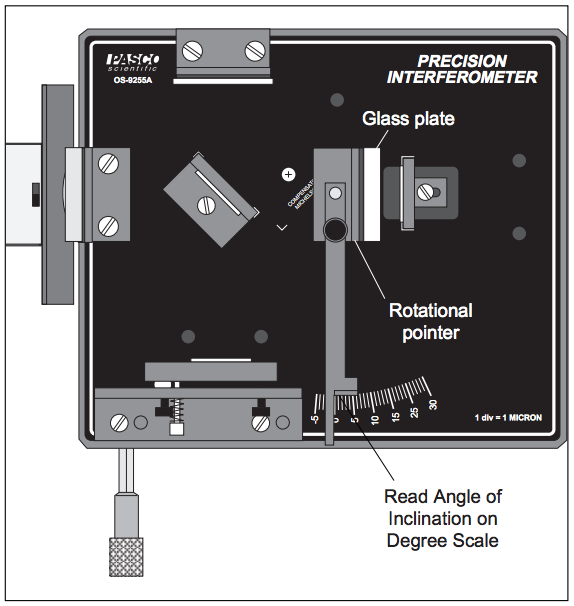
\includegraphics[scale=0.7]{equip3.png}
  \end{center}
  \caption{A diagram for the setup of Experiment 3. Since this setup is similar
    to the one from Experiment 1, only the components unique to Experiment 3
    have been labeled.}
\end{figure}

\begin{figure}[H]
  \label{tab:equip3List}
  \caption{A list of the equipment used in Experiment 3.}
  \begin{center}
    \begin{tabular}{|c|c|c|c|}
      \hline
      Manufacturer & Model & Serial Number & Specifications \\
      \hline
      PASCO Scientific & Precision Interferometer & OS-9255A & n/a \\
      PASCO Scientific & Laser Alignment Bench    & OS-9172  & n/a \\
      PASCO Scientific & Rotational Pointer       & OS-9256A & n/a \\
      PASCO Scientific & Rotating Table           & OS-9256A & n/a \\
      PASCO Scientific & Glass Plate              & OS-9256A & thickness: \SI{5}{\milli\meter} \\
      \hline
    \end{tabular}
  \end{center}
\end{figure}

\subsection{Procedures}

\qq Before beginning, ensure the interferometer is in Michelson mode and that it
is properly calibrated. Place the rotating table between the beam-splitter and
movable mirror, then attach the glass plate to the magnetic backing of the
rotational pointer. Position the rotational pointer so that it is pointing at
the zero degree marking on the base of the interferometer. 

\qq To ensure the plate is perpendicular to the optical path, remove the lens
from in front of the laser and hold the viewing screen in between the glass
plate and the movable mirror. Adjust the rotating table, while keeping the
rotational pointer in place, until there is one bright dot on the viewing
screen. Replace the lens once the plate in calibrated. 

\qq Slowly rotate the table by moving the rotational pointer and count the
number of fringes passing the reference point as the table is rotated from 0
degrees to at least 10 degrees. In our experiment, sufficiently many fringes
were counted up to an angle of 5 degrees.

\subsection{Data and Analysis}

\begin{figure}[H]
  \label{tab:exp3Data}
  \caption{The total number of fringes counted, \(N\), after the rotational
    pointer had been rotated \(\theta\) degrees.}
  \begin{center}
    \begin{tabular}{|c|c|}
      \hline
      Angle Displacement (\(\theta\)) (degrees) & Fringes Passed (\(N\)) \\
      \hline
      5 \(\pm\) 0.5 & 100 \\
      \hline
    \end{tabular}
  \end{center}
\end{figure}

\qq The index of refraction of the glass can be found with Equation
\ref{eqn:indexRefGlass} where
\(t = 5 \si{\milli\meter} \pm \SI{0.5}{\milli\meter}\) and
\(\lambda_0 = \SI{633}{\nano\meter}\),

\begin{align*}
  n_g &= \frac{(2 t - N \lambda_0) (1 - \cos{(\theta)})}{2 t (1 - \cos{(\theta)})
  - N \lambda_0} \\
  n_g &= \frac{\left( 2 (\num{5e-3}) - (100) (\num{633e-9}) \right) \left( 1 -
        \cos{(\SI{5}{\degree})} \right)}{ 2 (\num{5e-3}) \left( 1 -
        \cos{(\SI{5}{\degree})} \right) - (100) (\num{633e-9}) } \\
  n_g &= \num{1.50} \\
\end{align*}

\qq In order to find the error in the index of refraction, \(\delta n\),
Equation \ref{eqn:genErrProp} can be applied to Equation
\ref{eqn:indexRefGlass}. First, Equation \ref{eqn:indexRefGlass} can be
rewritten as a more easily differentiable function,

\begin{equation}
  \label{eqn:diffIndexRefGlass}
  n_g(t,\theta) = 3 - 2 cos{(\theta)} - N \lambda_0 \frac{1}{t} + N
    \lambda_0 \frac{1}{t} \cos{(\theta)} - \frac{1}{\cos{(\theta)}} - \frac{2}{N
    \lambda_0} t + \frac{2}{N \lambda_0} t \cos{(\theta)} \\
\end{equation}

Equation \ref{eqn:diffIndexRefGlass} can then be derived with respect to both
\(t\) and \(\theta\) to be later used in Equation \ref{eqn:genErrProp},

\begin{align*}
  \frac{\partial n_g}{\partial t} &= N \lambda_0 \frac{1}{t^2} - N \lambda_0
                                  \frac{1}{t^2} \cos{(\theta)} - \frac{2}{N
                                  \lambda_0} + \frac{2}{N \lambda_0} \cos{(\theta)} \\
\begin{split}  
  \frac{\partial n_g}{\partial t} &= 2 \sin{(\SI{5}{\degree})} - (100)
  (\num{633e-9}) \frac{1}{(\num{5e-3})} \sin{(\SI{5}{\degree})} - \\ &
  \tan{(\SI{5}{\degree})} \sec{(\SI{5}{\degree})} - \frac{2}{(100)
    (\num{633e-9})} (\num{5e-3}) \sin{(\SI{5}{\degree})} \\
  \end{split}\\
\frac{\partial n_g}{\partial t} &= -123
\end{align*}

\begin{align*}
  \frac{\partial n_g}{\partial \theta} &= 2 \sin{(\theta)} - N \lambda_0
  \frac{1}{t} \sin{(\theta)} - \tan{(\theta)} \sec{(\theta)} - \frac{2}{N
    \lambda_0} t \sin{(\theta)} \\
  \begin{split}
    \frac{\partial n_g}{\partial \theta} &= 2 \sin{(\SI{5}{\degree})} - (100)
    (\num{633e-9}) \frac{1}{(\num{5e-3})} \sin{(\SI{5}{\degree})} - \\ &
    \tan{(\SI{5}{\degree})} \sec{(\SI{5}{\degree})} -
    \frac{2}{(100)(\num{633e-9})} (\num{5e-3}) \sin{(\SI{5}{\degree})} \\
  \end{split} \\
  \frac{\partial n_g}{\partial \theta} &= -13.7 \\
\end{align*}

Now, the error of the index of refraction can be found with

\begin{align*}
  \delta n_g &= n_g \sqrt{\left( \frac{\partial n}{\partial t} \delta t \right) ^ 2 +
             \left( \frac{\partial n}{\partial \theta} \delta \theta \right) ^ 2} \\
  \delta n_g &= (1.5) \sqrt{\left( (-123) (\num{0.5e-3}) \right) ^ 2 + \left( (-13.7)
  (0.5) \right) ^ 2} \\
  \delta n_g &= 10.3 \\
\end{align*}

\subsection{Conclusion}

\qq The index of refraction of the glass was found to be
\(n_g = 1.50 \pm 10.3\). Although the value of the index of refraction of the
glass is a reasonable value of 1.5, the error is quite unreasonable. This error
most likely arose from miscalibration of the interferometer. Since more than
sufficiently many fringes were counted long before the recommended minimum angle
of \SI{10}{\degree}, it is probable that something was significantly misaligned.

%-----------END EXPERIMENT 3-----------

\end{document}
